\chapter{Konzept}

\begin{figure}
	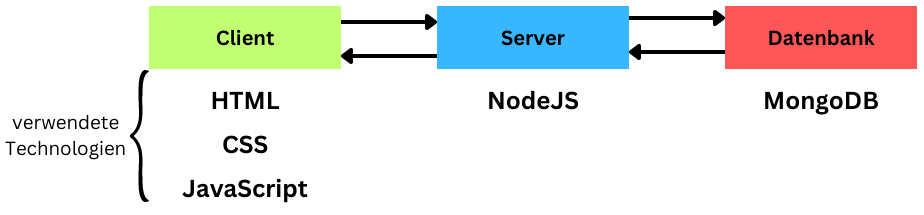
\includegraphics[width=\textwidth]{images/Architektur.png}
	\caption{Grobe Architektur des Systems}
\end{figure}

\begin{figure}
	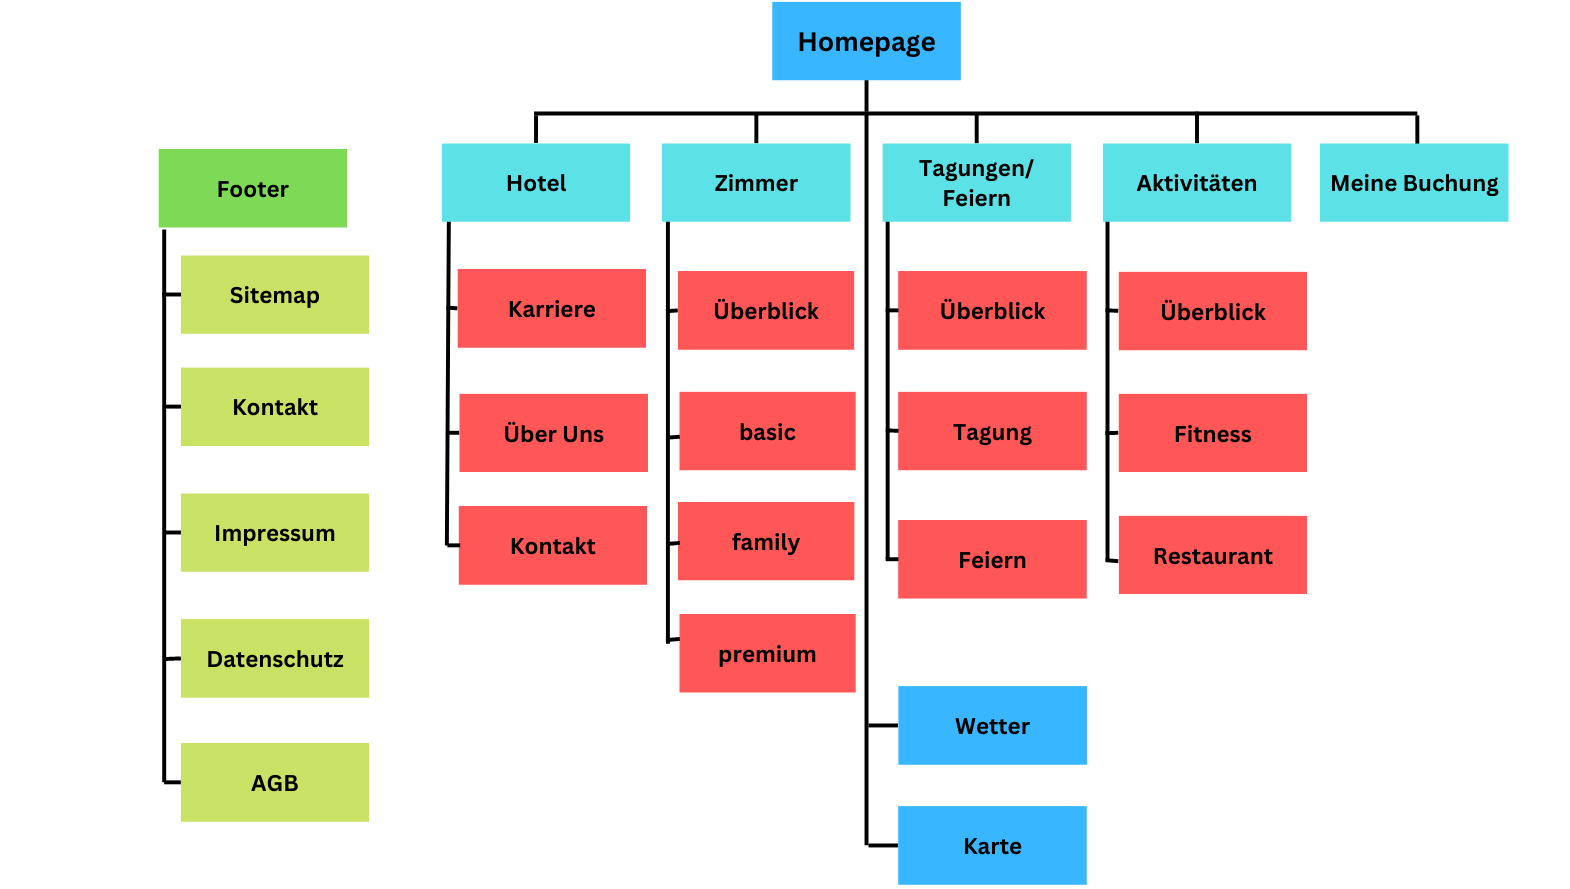
\includegraphics[width=\textwidth]{images/Sitemap.png}
	\caption{Sitemap}
\end{figure}

\begin{figure}
	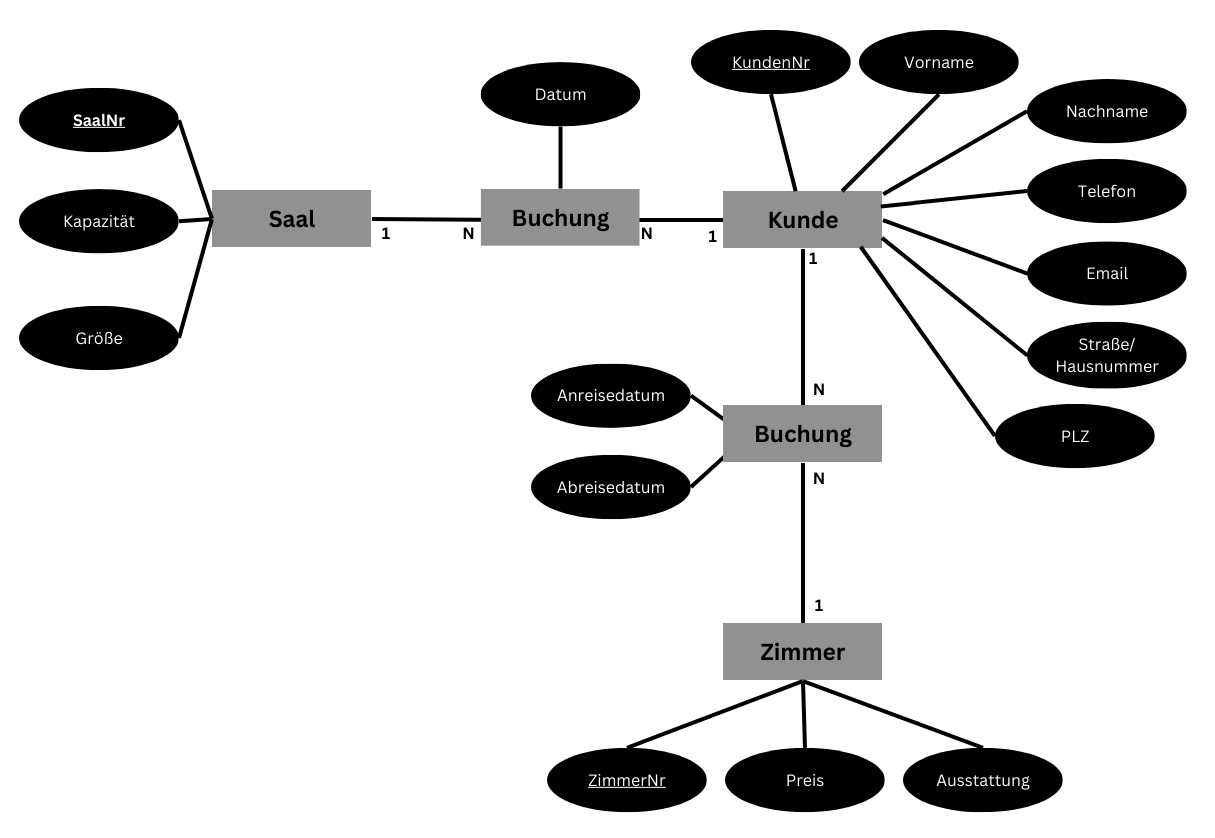
\includegraphics[width=\textwidth]{images/Datenbank.png}
	\caption{Datenbankentwurf}
\end{figure}

\begin{algorithm}
	\caption{Algorithmus um alle verfügbaren Räume zu erhalten}\label{alg:one}
	\KwData{rooms = alle Räume,
		reservations = alle Buchungen,
		arrival = Anreisedatum,
		departure = Abreisedatum
	}
	\KwResult{available = verfügbare Räume}
	$notAvailable \gets [\thinspace]$; \newline
	\For{room of rooms}{
		\For{reservation of reservations}{
			\If{$(room.id == reservation.room) \thickspace \&\& \thickspace !(departure < reservation.arrival \thickspace || \thickspace arrival > reservation.departure)$}{
				notAvailable.push(room);\newline
				break;
			}
		}
	}

    \Return{$available = rooms.filter(item \thickspace => \thickspace !notAvailable.includes(item))$}
\end{algorithm}